\section{OpenGL - podstawy}

OpenGL (\textit{Open Graphics Library}) stanowi otwarty i~uniwersalny interfejs umożliwiający renderowanie grafiki 2D i~3D. Obliczenia realizowane są dzięki bezpośredniej interakcji z~GPU, który, mając zaimplementowane potrzebne operacje, może szybko przeprowadzać obliczenia. Natura abstrakcyjnego interfejsu jakim jest OpenGL pozwala tworzyć przenośne programy renderujace grafikę bez zważania na platformę uruchomienia, gdzie obliczenia mogą być realizowane programowo jak i~sprzętowo.

\subsection{Bazowa aplikacja}
Biblioteką, która tworzy środowisko uruchomieniowe dla wyświetlania wyrenderowanej grafiki i~realizuje operacje wejścia-wyjścia jest GLUT (\textit{OpenGL Utility Toolkit}). Prosty program wyświetlajacy okno można stworzyć niewielkim nakładem pracy.

\begin{lstlisting}[language=C++, caption=Bazowy program wyświetlający czarne okno.]
#include <GL/glut.h>
void draw()
{
  glClearColor(0, 0, 0, 1);
  glClear(GL_COLOR_BUFFER_BIT);
  glFlush();
}

int main(int argc, char **argv)
{
  glutInit(&argc, argv);
  glutInitDisplayMode(GLUT_SINGLE | GLUT_RGB);
  glutInitWindowPosition(50, 50);
  glutInitWindowSize(800, 800);
  glutCreateWindow("Lab GK");
  glutDisplayFunc(draw);
  glutMainLoop();
  return 0;
}
\end{lstlisting}

W funkcji \lstinline{main} w pierwszej kolejności inicjalizowana jest sama aplikacja, a następnie wszystkie jej parametry. Następnie do biblioteki GLUT przekazywana poprzez wskaźnik jest funkcja \lstinline{draw}, ktora jest odpowedzialna za bezpośrednią interakcję z API OpenGL, a zatem za rysowanie właściwych elementów w wyświetlonym oknie. W tej wersji funkcja \lstinline{draw} czyści okno kolorem czarnym i opróżnia bufor przekazując dane na ekran.

\subsection{Dywan Sierpińskiego}
Dywan Sierpińskiego jest jest fraktalem otrzymanym z kwadratu podzielonego na 9 mniejszych kwadratów, z których usuwany jest środkowy. Procedura ta jest rekurencyjnie powtarzana dla pozostałych ośmiu kwadratów.
\begin{figure}[h]
  \centering
  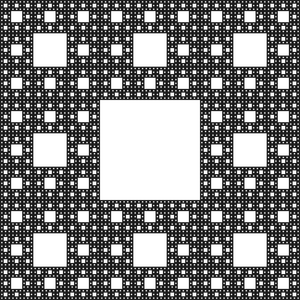
\includegraphics[width=0.3\linewidth]{img/300px-Sierpinski6.png}
  \caption{Dywan Sierpińskiego po 6 iteracjach.}
\end{figure}

\subsubsection{Rysowanie rekurencyjne}
Rysowanie dywanu Sierpińskiego zrealizowane za pomocą rekurencji zakłada rekurencyjne wywołanie funkcji dla każdego z ośmiu zewnętrznych kwadratów fraktalu. Poziomów wywoływań następuje tyle ile zostało zdefiniowane dla pierwszego wywołania funkcji. Gdy zostanie spełniony warunek zakończenia rekurencji, rysowany jest kwadrat. Funkcja po raz pierwszy zostaje wywołana w metodzie \lstinline{draw} zaraz po wyczyszczeniu okna.

\begin{figure}[H]
  \
  \begin{minipage}[t]{.45\linewidth}
      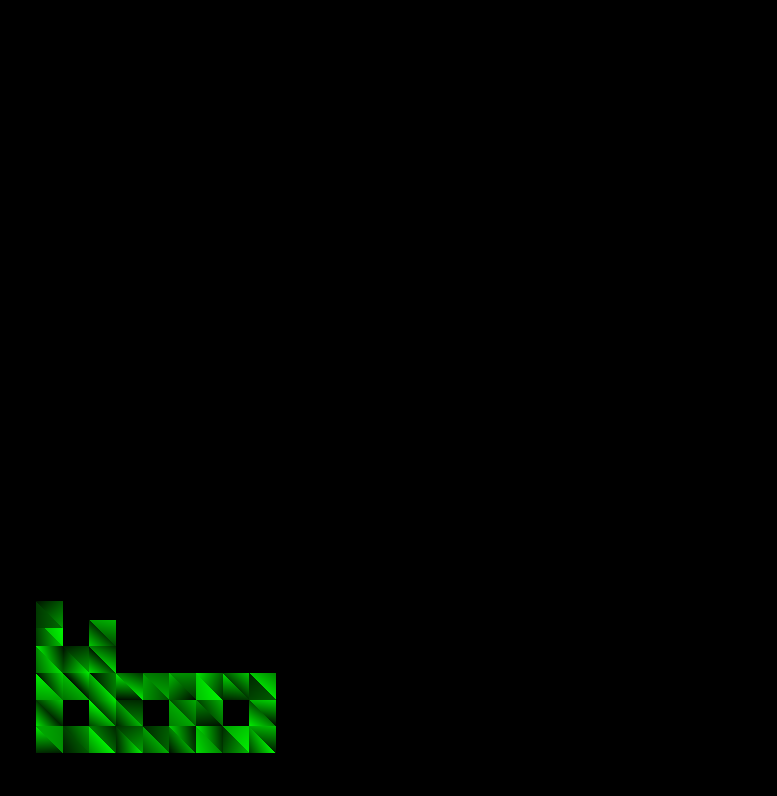
\includegraphics[width=\linewidth]{img/serpinski_3_s1.png}
      \caption{Częściowo narysowany dywan Sierpińskiego po zakończeniu 30 gałęzi rekurencji.}
  \end{minipage}
  \hspace{.05\linewidth}
  \begin{minipage}[t]{0.45\linewidth}
      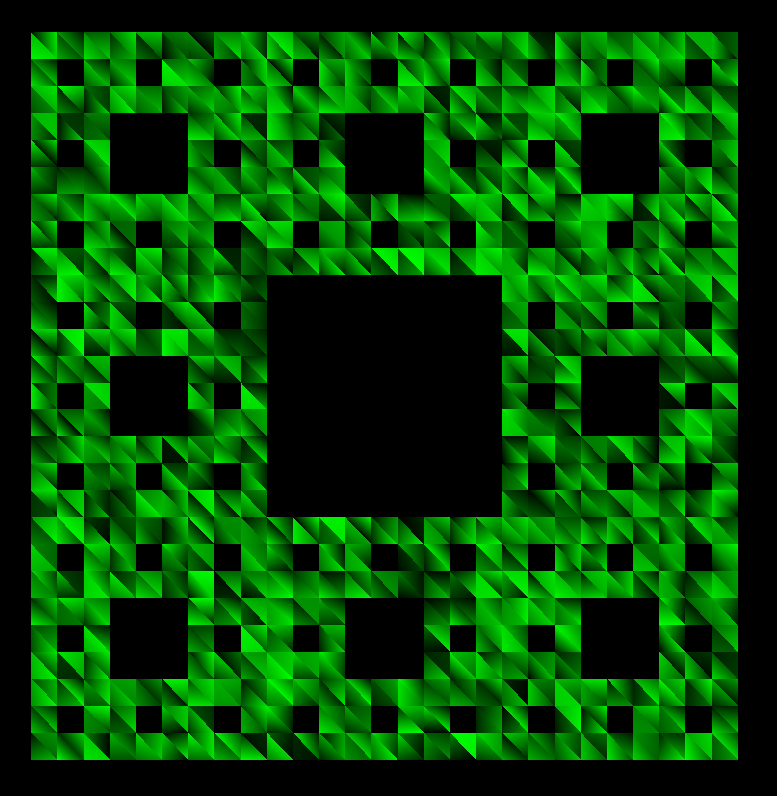
\includegraphics[width=\linewidth]{serpinski_3_s2}
      \caption{Dywan Sierpińskiego narysowany w całości.}
  \end{minipage}
\end{figure}

\begin{lstlisting}[language=C++, caption=Funkcja rysująca dywan Sierpińskiego rekurencyjnie. Pominięto niektóre wywołania.]
void carpet(int levels, float a, float dx = 0, float dy = 0)
{
  if (levels != 0)
  {
    a = a / 3;
    carpet(levels - 1, a, dx - a, dy - a);
    ...
    carpet(levels - 1, a, dx + a, dy + a);
  }
  else
  {
    //Pomocnicza funkcja rysujaca kwadrat
    rect(dx, dy, a); 
  }
}
\end{lstlisting}
\subsubsection{Rysowanie iteracyjne}
Rysowanie iteracyjne możliwe jest do osiągnięcia przez matematyczne sprawdzenie czy dany kwadrat ma być wypełniony czy nie, albo zamianę wersji rekurencyjnej do wersji iteracyjnej z wykorzystaniem kolejki i struktury danych opisującej aktualny poziom rysowania.

\begin{lstlisting}[language=C++, caption=Struktura danych przechowująca aktualny stan rysowania.]
struct CarpetLevelData
{
  int level;
  float a;
  float dx = 0;
  float dy = 0;
};
\end{lstlisting}


\begin{lstlisting}[language=C++, caption=Funkcja rysująca dywan Sierpińskiego iteracyjnie. Pominięto niektóre wywołania.]
void carpetIt(int levels, float a)
{
  queue<CarpetLevelData> q = queue<CarpetLevelData>();
  q.push({levels, a});
  while (!q.empty())
  {
    CarpetLevelData data = q.front();
    if (data.level > 0)
    {
      data.a = data.a / 3;
      q.push({data.level - 1, data.a, data.dx - data.a, data.dy - data.a});
      ...
      q.push({data.level - 1, data.a, data.dx + data.a, data.dy + data.a});
    }
    else
    {
      rect(data.dx, data.dy, data.a);
    }
    q.pop();
  }
\end{lstlisting}

\subsubsection{Losowe kolory i perturbacje}
Losowe kolory osiągnięto poprzez wywołanie funkcji \lstinline{glColor3ub(0, randChar(), 0)} przed wywołaniem funkcji interfejsu OpenGL definiującą składowy wierzchołek trojąta tworzącego kwadrat, gdzie funkcja \lstinline{randChar} zwraca liczbę z przedziału $<0;255>$. Mając kontrolę nad rysowanem każdego kwadratu można wprowadzić również losowe jego przesunięcie w osi X i Y.

\begin{figure}[h]
  \centering
  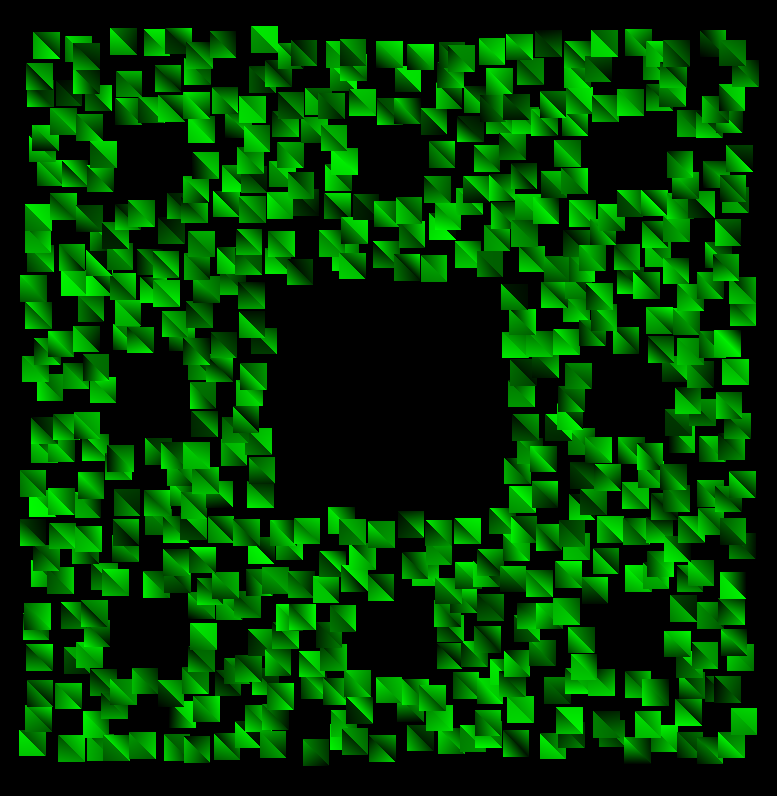
\includegraphics[width=0.4\linewidth]{img/serpinski_3_s3.png}
  \caption{Dywan Sierpińskiego po 3 iteracjach z losowym kolorem zielonym oraz perturbacjami.}
\end{figure}